\documentclass{article}

\usepackage[utf8]{inputenc}
\usepackage[spanish]{babel}
\usepackage{babelbib}
\usepackage{geometry}
\usepackage{mathtools}
\usepackage{graphicx}
\usepackage{float}

\geometry{letterpaper,tmargin=2cm,bmargin=2cm,lmargin=2cm,rmargin=2cm}

\begin{document}

\begin{titlepage}
    \centering
    \vspace{2cm}

    {\huge\bfseries Análisis de un sistema no lineal para el tratamiento del VIH\par}
    \vspace{5cm}
    {\Large\itshape Alejandro Salgado Gómez\par}
    \vfill

    Profesor\par
    {\large Santiago Lopez Restrepo\par}

    \vfill

    {\large Modelación y simulación IV \par}
    \vspace{0.2cm}
    {\large Ingeniería Matemática \par}
    \vspace{0.2cm}
    {\large Departamento de ciencias matemáticas \par}
    \vspace{0.2cm}
    {\large Escuela de ciencias \par}
    \vspace{0.2cm}
    {\large Universidad EAFIT \par}

    \vfill

    {\large Noviembre 22 de 2017}
\end{titlepage}


\section{Planteamiento del problema}

Las estrategias para contrarrestar el VIH utilizando métodos de control están
recibiendo cada vez más atención. Estudios detallados que combinan
técnicas de modelado con resultados clínicos muestran que la fase inicial de la
infección puede ser representada utilizando modelos no lineales simples.\cite{paper}
Este hecho impulsó la producción de artículos donde se trabaja con los principios
de control con el fin de estudiar diversas estrategias para implementar terapias de dicha
enfermedad.\\

En \cite{model} se encontró un modelo no lineal con tres variables de estado, en el
cual la dinámica de una de sus variables puede ser calculada por medio de una
ecuación algebráica al asumir su cambio como instantáneo en reacción a las variaciones
de otra variable, reduciendo así el modelo a uno de dos estados.

Este modelo asume la complejidad no lineal para representar de una manera
mas acertada el efecto que las drogas usadas en el tratamiento de esta
enfermedad tienen en los pacientes, con el fin de buscar alternativas para
implementar estrategias de control en las terapias del VIH.\\

El problema que se desea abordar en este trabajo es el análisis en distintos niveles
de dicho modelo, con el objetivo de entender más a fondo su estructura y
funcionamiento, desde los detalles más generales hasta los más específicos.

\section{Objetivo general}

Analizar el sistema no lineal de ecuaciones diferenciales escogido, sus componentes y
como reacciona al cambiar sus condiciones con el propósito de aplicar la teoría
estudiada en clase.

\section{Objetivos específicos}

\begin{itemize}
    \item Reconocer parámetros, entradas y salidas del sistema escogido.
    \item Simular el sistema.
    \item Estudiar el acoplamiento de ecuaciones.
    \item Realizar un análisis completo de las gráficas.
    \item Análisis del sistema al variar entradas y condiciones iniciales.
    \item Hallar los puntos de equilibrio del sistema.
    \item Linealizar el sistema y hacer un análisis de estabilidad en los puntos de equilibrio.
\end{itemize}

\section{Antecedentes del modelo escogido}

Existen varios antecentes directamente relaciónados con el trabajo realizado en el
artículo, como lo son \cite{ieee1}, \cite{ieee2}, \cite{ieee3}. Sin embargo,
debido a la dificultad de conseguir dichos trabajos, se proponen como
antecedentes los siguientes modelos generales.

\newpage

    \subsection{Modelo SIR}

        \Large
        $$\dot{s} = -b s(t) i(t)$$
        $$\dot{i} = b s(t) i(t) - k i(t)$$
        $$\dot{r} = k i(t)$$
        \normalsize

        \vspace{0.5cm}

        \begin{tabular}[t]{|p{4cm} p{3.5cm}|}
            \hline
            \textbf{Variables de estado} & \textbf{Unidades} \\
            \hline
            $s$: Población susceptible & Número de individuos\\
            $i$: Población infectada  & Número de individuos\\
            $r$: Población recuperada & Número de individuos\\
            \hline
        \end{tabular}
        \hspace{0.5cm}
        \begin{tabular}[t]{|p{4cm} p{4cm}|}
            \hline
            \textbf{Parámetros} & \textbf{Unidades} \\
            \hline
            $b$: tasa de infección    & $1/(individuos * tiempo)$\\
            $k$: tasa de recuperación & $1/tiempo$\\
            \hline
        \end{tabular}
        \cite{sir}

        \vspace{0.5cm}

        En este modelo se busca plasmar la dinámica de tres poblaciones de
        individuos, los susceptibles, quienes todavía no han sido contagiados
        por el tipo de infección a modelar, los infectados y los recuperados,
        quienes ya son inmunes.\\

        La primera ecuación muestra el cambio en la población de
        susceptibles debido al contagio que producen los infectados, la
        segunda muestra como la población de los infectados varía
        dependiendo de la cantidad de contagiados y el número de recuperados, y
        por último en la tercera, se determina como es el proceso de cura
        de los individuos infectados.

    \subsection{Modelo predador-presa}

        \Large
        $$\dot{p} = \alpha p(t) - \beta p(t) d(t)$$
        $$\dot{d} = \lambda p(t) d(t) - \gamma d(t)$$
        \normalsize

        \vspace{0.5cm}

        \begin{tabular}[t]{|p{4cm} p{3.5cm}|}
            \hline
            \textbf{Variables de estado} & \textbf{Unidades} \\
            \hline
            $p$: Población presas       & Número de individuos\\
            $d$: Población depredadores & Número de individuos\\
            \hline
        \end{tabular}
        \hspace{0.5cm}
        \begin{tabular}[t]{|p{4.5cm} p{4cm}|}
            \hline
            \textbf{Parámetro} & \textbf{Unidades} \\
            \hline
            $\alpha$:  tasa nacimiento presas   & $1/tiempo$\\
            $\beta$:   tasa caza                & $1/(individuos * tiempo)$\\
            $\lambda$: tasa alimentación        & $1/(individuos * tiempo)$\\
            $\gamma$:  tasa muerte depredadores & $1/tiempo$\\
            \hline
        \end{tabular}
        \cite{predator}

        \vspace{0.5cm}

        En este modelo se tienen dos poblaciones, presas y depredadores, los
        cuales presentan un comportamiento de crecimiento exponencial en
        ausencia del otro (positivo para las presas y negativo para los
        predadores). En este modelo la primera ecuación muestra como el
        crecimiento exponencial de las presas es diezmado por la acción de los
        depredadores y la segunda ecuación define como la cantidad de presas
        removidas influye en el decrecimiento de la población de depredadores.

\newpage

\section{Modelo escogido}

    \Large
    $$\dot{x_1} = s -dx_1 - (1-u_1) \beta x_1 x_3$$
    $$\dot{x_2} = (1-u_1) \beta x_1 x_3 - \mu x_2$$
    $$\dot{x_3} = (1-u_2) k x_2 - c x_3$$
    \normalsize

\vspace{1cm}

    \begin{tabular}{|p{6cm} p{2.5cm}|}
        \hline
        \textbf{Variables de estado} & \textbf{Unidades} \\
        \hline
        $x_1$: Concentración de células saludables & $celulas / mm^3$\\
        $x_2$: Concentración de células infectadas & $celulas / mm^3$\\
        $x_3$: Concentración de virus libre        & $copias / mm^3$\\
        \hline
    \end{tabular}

    \vspace{0.5cm}

    \begin{tabular}{|p{8cm} p{2.5cm}|}
        \hline
        \textbf{Entradas} & \textbf{Unidades} \\
        \hline
        $u_1$: Eficiencia para prevenir la infección              & Adimensional \\
        $u_2$: Eficiencia para evitar la creacion de virus libres & Adimensional \\
        \hline
    \end{tabular}

    \vspace{0.5cm}

    \begin{tabular}{|p{7cm} p{2cm} c|}
        \hline
        \textbf{Parámetro} & \textbf{Valor} & \textbf{Unidades} \\
        \hline
        $d$: Tasa de muerte natural de las células      & 0.02            & $s^{-1}$\\
        $k$: Tasa de producción de virus libres         & 100             & $s^{-1}$\\
        $s$: Tasa de producción de células sanas        & 10              & $mm^{-3} s^{-1}$\\
        $\beta$: Tasa de infección                      & $2.4 * 10^{-5}$ & $mm^3 s^{-1}$\\
        $\mu$: Tasa de muerte de las células infectadas & 0.24            & $s^{-1}$\\
        $c$: Tasa de muerte de los virus libres         & 2.4             & $s^{-1}$\\
        \hline
    \end{tabular}

\vspace{1cm}

En este modelo se busca plasmar la dinámica del virus VIH con el uso de tres
variables de estado que representan las células saludables, las infectadas y la
concentración de células libres en el cuerpo.\\

En la primera ecuación se muestra la dinámica de las células sanas y como su
disminución se ve afectada tanto por su muerte natural como por la influencia
del virus, en la segunda se expresa el cambio en las células
contaminadas como el contagio de células sanas menos una tasa de muerte natural
de células infectadas y por último en la tercera, se plasma el proceso
por el cual las células contaminadas liberan más virus en el sistema, los
cuales a su vez también tienen una tasa de muerte natural que los disminuye.\\

    \subsection{Modelo reducido}

    \Large
    $$\dot{x_1} = s -dx_1 - (1-u) \frac{\beta k}{c} x_1 x_2$$
    $$\dot{x_2} = (1-u) \frac{\beta k}{c} x_1 x_2 - \mu x_2$$
    \normalsize

    \vspace{0.5cm}

    \begin{tabular}{|p{6cm} p{2.5cm}|}
        \hline
        \textbf{Variables de estado} & \textbf{Unidades} \\
        \hline
        $x_1$: Concentración de células saludables & $celulas / mm^3$\\
        $x_2$: Concentración de células infectadas & $celulas / mm^3$\\
        \hline
    \end{tabular}

    \vspace{0.5cm}

    \begin{tabular}{|p{8.5cm} p{2.5cm}|}
        \hline
        \textbf{Entradas} & \textbf{Unidades} \\
        \hline
        $u$: esta entrada es usada para simplificar las ecuaciones del modelo,
             tiene un valor de $u_1+u_2-u_1 u_2$ & Adimensional \\
        \hline
    \end{tabular}

    \vspace{0.5cm}

    \begin{tabular}{|p{7cm} p{2cm} c|}
        \hline
        \textbf{Parámetro} & \textbf{Valor} & \textbf{Unidades} \\
        \hline
        $d$: tasa de muerte natural de las células      & 0.02            & $s^{-1}$\\
        $k$: tasa de producción de virus libres         & 100             & $s^{-1}$\\
        $s$: tasa de producción de células sanas        & 10              & $mm^{-3} s^{-1}$\\
        $\beta$: tasa de infección                      & $2.4 * 10^{-5}$ & $mm^3 s^{-1}$\\
        $\mu$: tasa de muerte de las células infectadas & 0.24            & $s^{-1}$\\
        $c$: tasa de muerte de los virus libres         & 2.4             & $s^{-1}$\\
        \hline
    \end{tabular}

    \cite{model}

    \vspace{0.5cm}

Este modelo es bastante similar al anterior, tanto en estructura como en
aplicación, se puede ver basicamente como su simplifación. Los cambios
realizados son, en primer lugar, la eliminación de $x_3$ como variable de
estado al encontrar que su cambio respecto a las variaciones de $x_2$ sucede de
manera casi instantánea, lo que permite prescindir de $x_3$ como variable de
estado al expresarla como una ecuación algebráica, reduciendo así el modelo a
segundo orden.  Y en segundo lugar, la combinación de $u_1$ y $u_2$ para formar una
nueva entrada, con el objetivo simplificar las ecuaciones y facilitar el
entendimiento del modelo.

\section{Análisis de las ecuaciones}

En esta sección se discutirá con mas detalle la estructura del modelo escogido
en su versión reducida, ya que es esta la que se usará para el resto del trabajo.

    \subsection{Proceso de reducción}

    el modelo pudo ser reducido al observar la relación que existe
    entre las variables $x_2$ y $x_3$, donde después de un periodo corto de
    tiempo se vuelven proporcionales, tal como se muestra en la figura \ref{fig:relacion}.

    Ahora, la ecuación 3 puede ser vista como un sistema lineal estable con
    $x_2$ como entrada, en donde la estabilidad se alcanza rápidamente, por lo
    que al hacer $\dot{x_3} = 0$ se obtiene

    \Large
    $$x_3 = (1-u_2) \frac{k}{c} x_2$$
    \normalsize

    Y luego de reemplazar esta expresión en las otras dos ecuaciones se obtiene el
    modelo reducido con una entrada $u = u_1 + u_2 - u_1 u_2$.

    \begin{figure}[h!]
        \centering
        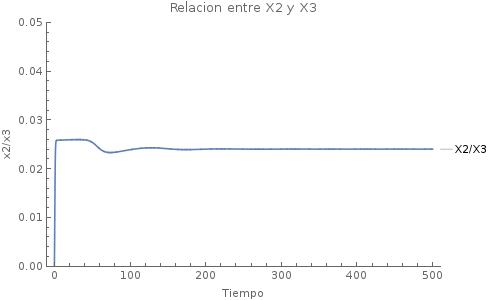
\includegraphics[scale=0.5]{Images/Vih-x2-x3}
        \caption{Relación entre las variables $x_2$ y $x_3$.}
        \label{fig:relacion}
    \end{figure}

    \newpage

    \subsection{Suposiciones e información general del modelo}

    El modelo tiene pocas suposiciones, la principal de ellas es tomar todos
    párametros como constantes, tal como la tasa de producción y muerte de las
    células sanas e infectadas, o las tasas de produccion y muerte de virus libres.

    Además de esto, aunque no es una suposición, el modelo plantea que no es
    posible eliminar la infección por completo, característica que se esperaría
    en un caso real de la enfermad.\\

    Es importante mencionar que el modelo se puede trabajar tanto para
    individuos infectados como para aquellos que se ecuentran sanos, esto dependiendo
    de si el valor de la variable $x_2$ es distinta de cero o no, respectivamente.
    Aunque se espera que sea utilizado en situaciones de infección, ya que de lo
    contrario las dinámicas que se generan no son tan interesantes.\\

    Ahora, de entre la información general del modelo se puede destacar
    la similitud con los modelos propuestos como antecedentes, específicamente
    en aspectos como la reducción de las poblaciones debido a la infección, su
    contagio y la muerte de los virus, tal como en el modelo SIR, y en la
    decaída de la poblaciones por una tasa de muerte, donde se puede ver cierta
    similitud con el modelo predador-presa.

    En segundo lugar es importante resaltar como las tasas de infección de las
    células sanas y la tasa de creación de virus libres pueden ser
    influenciadas con el efecto de drogas que afecten el desarrollo del virus.
    Dicha influencia se modela con las variables de entrada, donde $u_1$
    toma valores entre 0 y 1, representando la eficiencia de drogas ITR
    (Inhibidores de la Transcriptasa Inversa) que pueden reducir la propagación
    del virus. Y la variable $u_2$, que toma valores en el mismo intervalo, y
    representa la acción de drogas PI (Inhibidores de proteasa), las cuales
    previenen que las células infectadas produzcan más virus libres,
    permitiendo así ejercer un control sobre el desarrollo del virus en el
    cuerpo.\\

    Cabe resaltar también, que en la actualidad ninguna droga llega a una
    eficiencia del 100\% por lo cual un valor cercano a 1 en las entradas que
    representan su efecto ocasiona que la simulación tome una condición cada vez
    más teórica.\cite{model}\\

    Finalmente, aunque aun no es tratado de manera detallada en este trabajo,
    existen otros modelos relacionados como el presentado en \cite{ieee4},
    los cuales en las secciones de control tienen suposiciones de linealidad en
    algunas de las variables que manipulan, mientras que en este modelo la
    dependencia del control no es lineal, lo que conlleva a un trabajo de álgebra
    mas complicado, pero permite representar de una manera mas acertada la
    situación que se desea modelar.\\

    \subsection{Acoplamiento de ecuaciones y parámetros}

    Tal como se mencionó anteriormente, la descripción del modelo reducido es
    similar a la que se dio del modelo original en una sección anterior, sin
    embargo, en esta parte se describirán con mas detalle los componentes de las
    ecuaciones que describen el comportamiento del sistema con mas detalle.\\

    En primer lugar se tiene la ecuación que representa el cambio de la
    concentración de células sanas, en esta ecuación se tienen tres términos,
    el primero es la producción de células sanas que tiene la persona, a las
    cuales se les resta el segundo término, que representa la cantidad de
    células que mueren por causas naturales. Finalmente, se tiene la parte de la
    ecuación que da información sobre la tasa de infección, esta tasa es
    proporcional al producto de $x_1$ y $x_3$, pero debido a la reducción del
    modelo queda expresado como una relación entre $x_1$ y $x_2$, donde se
    tiene un factor que relaciona la tasa de producción y muerte de células
    libres con el resto del término, y de manera análoga al primer modelo se
    tiene otro factor que integra los efectos de medicamentos en el desarrollo
    del virus.

    En segundo lugar se tiene la ecuación que representa el cambio en la concentración
    de células infectadas, proceso que esta expresado como la diferencia entre el
    último término de la primera ecuación, el cual representa su crecimiento, y
    la cantidad de células infectadas que mueren.

    Finalmente, se puede observar claramente el acoplamiento entre las ecuaciones
    debido a la utilización del mismo término tanto para calcular la reducción de las
    células sanas en la primera ecuación, como el crecimiento del número
    de céluas infectadas en la segunda, generando así una fuerte dependencia entre
    las dos ecuaciones.

\newpage

\section{Diagrama de estados}

\begin{figure}[h!]
    \centering
    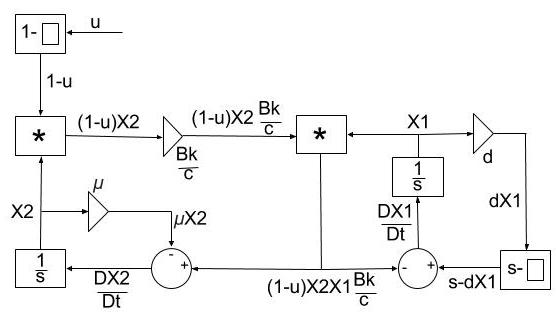
\includegraphics[width=\textwidth]{Images/State-diagram.jpeg}
    \caption{Diagrama de estados.}
    \label{fig:state-diagram}
\end{figure}

En este diagrama $s -$ y $1-$ representan las operaciones de sumar el negativo
de su entrada al valor de $s$ y $1$ respectivamente, $*$ representa la
multiplicación de dos entradas y $\frac{1}{s}$ representa un integrador.

\section{Simulaciones}

Las siguientes simulaciones fueron realizadas con la ayuda del software Mathematica
\cite{mathematica}, el código usado puede ser encontrado en
https://github.com/AlejandroSalgadoG/Miscellaneous/tree/master/Mathematica/VIH.

\begin{itemize}
    \item Modelo con entrada constante.
    \item Modelo con variación en las entradas.
    \item Modelo con diferentes condiciones iniciales.
    \item Trayectorias de estado con condiciones iniciales aleatorias.
\end{itemize}

Los valores que se utilizaron en cada simulación se presentan en el lado
izquierdo de las imágenes. los primeros dos valores corresponden a las
condiciones iniciales de $x_1$ y $x_2$ respectivamente, el siguiente valor
corresponde a la entrada, y finalmente el tercer campo da información sobre el
tiempo en el cual la entrada sufre la modificación especificada en el último
campo de la ventana. Es importante mencionar que este último campo corresponde al valor
total de la entrada, no a una desviación.

\newpage

\begin{figure}[H]
    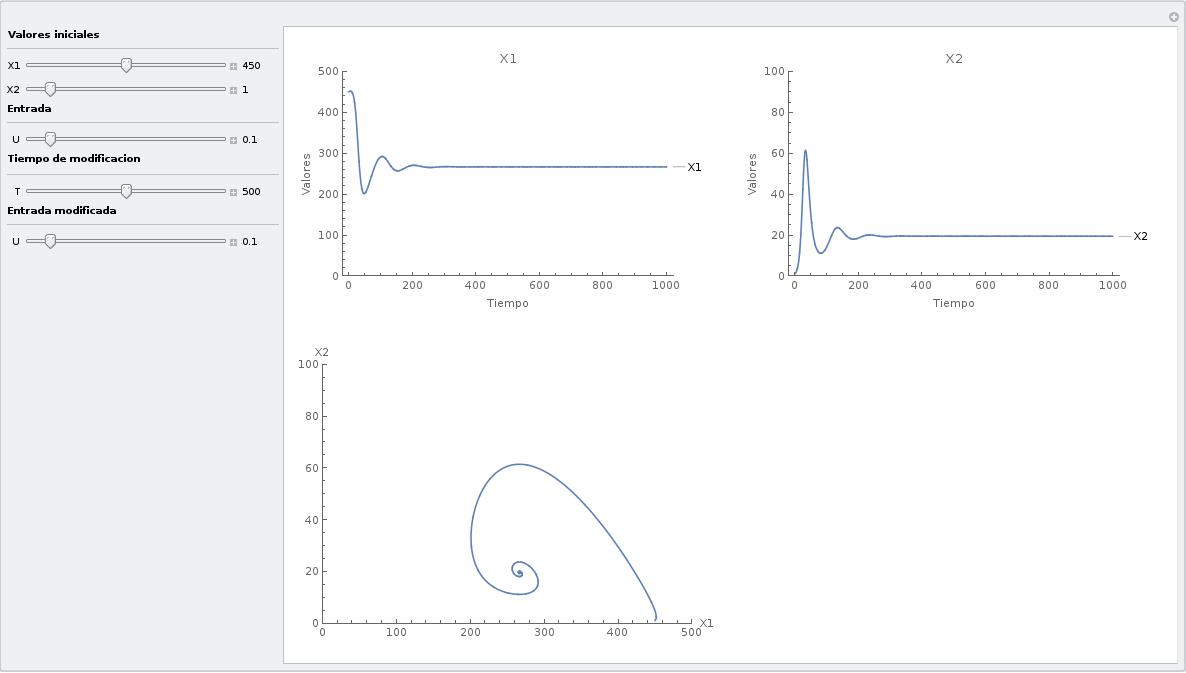
\includegraphics[width=\textwidth]{Images/Vih-u-constante}
    \caption{Simulación con entradas constantes.}
\end{figure}

En esta simulación se muestra el comportamiento del sistema con entrada constante,
tal como se puede ver en las gráficas el sistema presenta una oscilación inicial
que representa el crecimiento de las células infectadas y el decremento de las
células sanas hasta llegar a un punto de equilibrio donde las dos poblaciones se
estabilizan.

\begin{figure}[H]
    \centering
    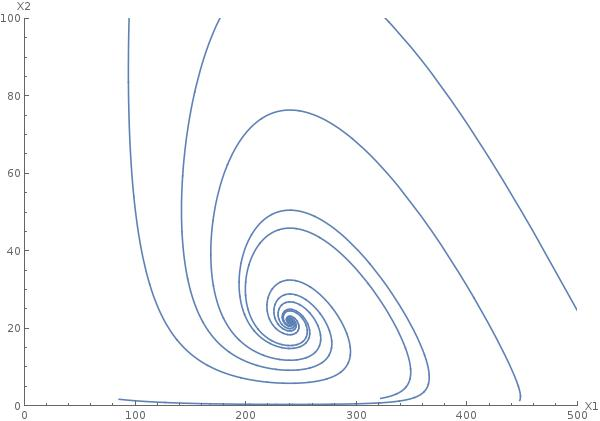
\includegraphics[scale=0.4]{Images/Vih-random}
    \caption{Trayectorias de estado con condiciones iniciales aleatorias.}
\end{figure}

En este diagrama se muestran varias trayectorias de estado desde distintas
condiciones iniciales, con la entrada constante, a partir de esta gráfica se
puede observar como el sistema tiende a presentar un comportamiento oscilante al
inicio de las simulaciones, representado en los giros que se dan el plano,
las cuales van disminuyendo hasta converger a un punto estable.

\begin{figure}[H]
    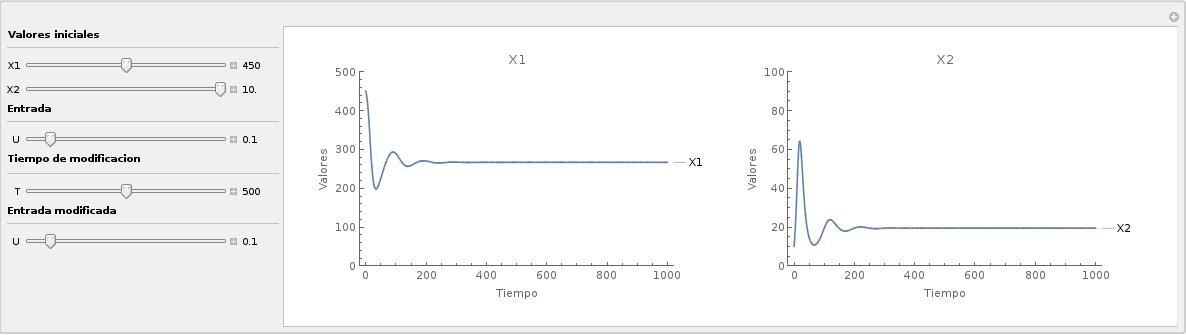
\includegraphics[width=\textwidth]{Images/Vih-more-infected.jpeg}
    \caption{Simulación con un incremento en la cantidad de células infectadas iniciales.}
\end{figure}

Basado en lo mostrado en esta simulación se puede ver como al incrementar el
número de células infectadas que el modelo tiene inicialmente, los picos de
las variables de estado se generan un poco más rapido, lo cual se puede interpretar como una
reacción mas acelerada de crecimiento de en las células infectadas y un
decrecimiento en las células sanas.

\begin{figure}[H]
    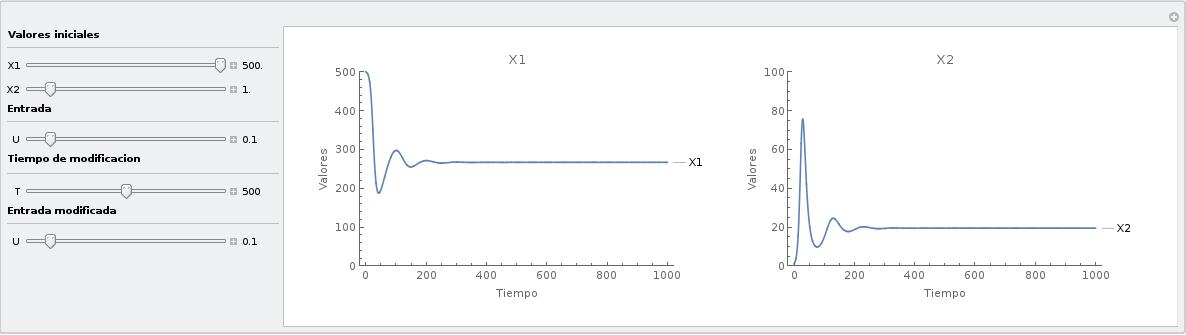
\includegraphics[width=\textwidth]{Images/Vih-more-healthy.jpeg}
    \caption{Simulación con un incremento en la cantidad de células sanas iniciales.}
\end{figure}

Se puede observar que en el caso de aumentar el número de células sanas, se obtienen
picos mas elevados al inicio de la simulación, lo cual se puede interpretar como
una reacción mas agresiva en cuanto al cambio el número tanto de las células infectadas
como de las sanas.

\begin{figure}[H]
    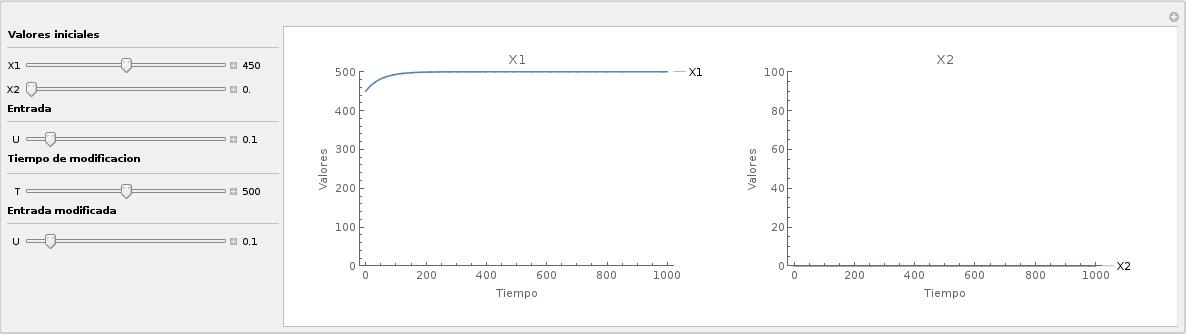
\includegraphics[width=\textwidth]{Images/Vih-healthy.jpeg}
    \caption{Simulación de una persona sana.}
\end{figure}

Tal como es de esperarse, en el caso de que la persona no este infectada las células
sanas pueden reproducirse sin problemas, siendo capaces de aumentar su número hasta
estabilizarse, mientras que la población de células infectadas se mantiene
en cero.

\begin{figure}[H]
    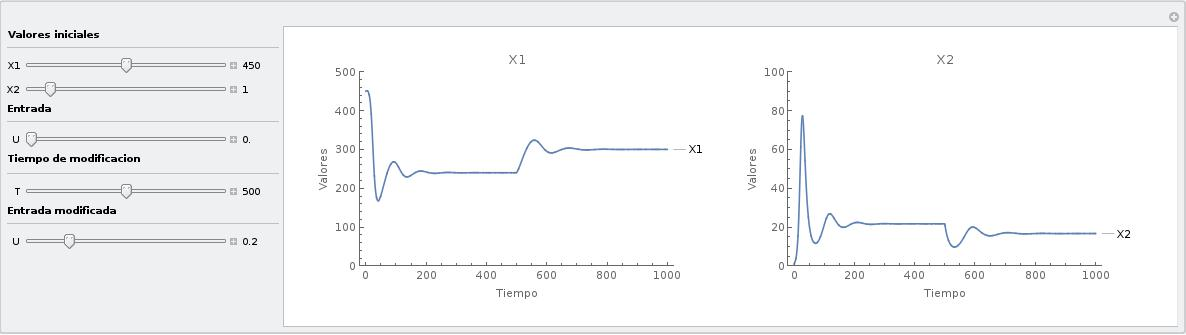
\includegraphics[width=\textwidth]{Images/Vih-noinput-input.jpeg}
    \caption{Simulación con entrada nula que se incrementa.}
\end{figure}

Las siguientes simulaciones tienen el objetivo de ver el comportamiento del
sistema al variar su entrada. En este caso se tiene una simulación en la que
el paciente no recibe medicamentos en un inicio, pero luego de un tiempo se comienza
a suministrar una dosis. El resultado de esta variación es una oscilación en ambas
poblaciones de células que converge en un incremento en el número
de las células sanas y un decremento leve en el número de las infectadas.

\begin{figure}[H]
    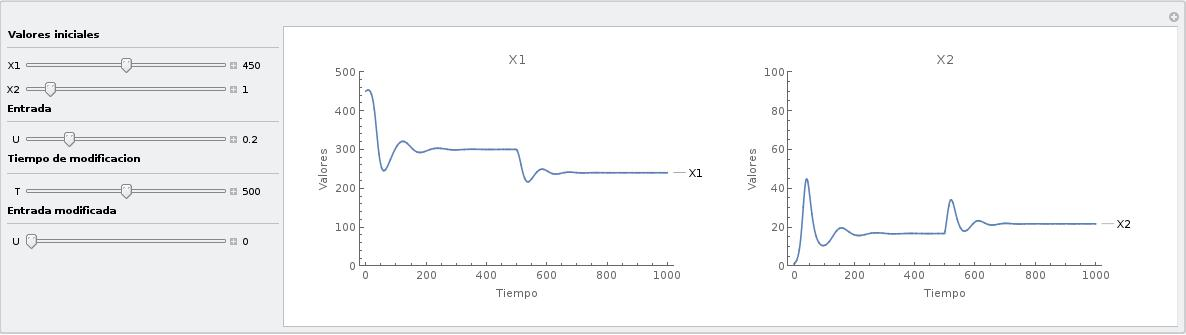
\includegraphics[width=\textwidth]{Images/Vih-input-noinput.jpeg}
    \caption{Simulación con decremento en la entrada.}
\end{figure}

En este caso se observa una simulación en la que la persona analizada recibe
medicamentos en un principio pero luego se dejan de suministrar. Como es de esperarse
luego de una característica oscilación el número de células sanas se disminuye
y el número de células infectadas se incrementa.

\begin{figure}[H]
    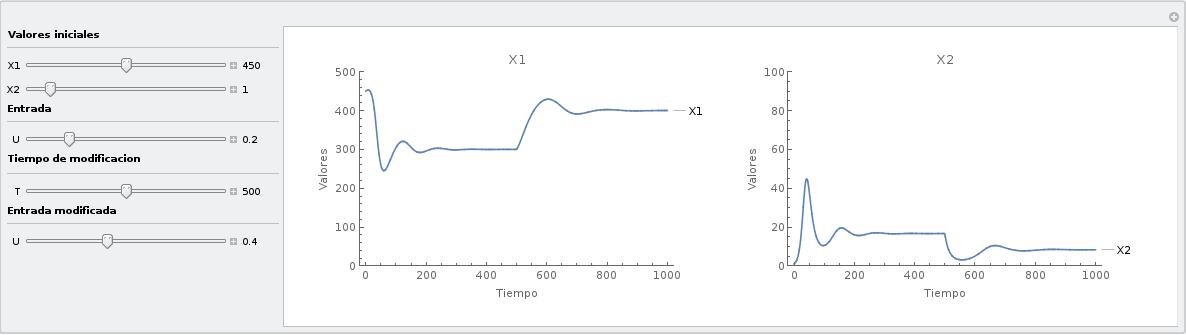
\includegraphics[width=\textwidth]{Images/Vih-input-moreinput.jpeg}
    \caption{Simulación con incremento en la entrada.}
\end{figure}

Por último, en esta simulación se puede observar el caso en el que se
suministran medicamentos desde el principio y luego de un tiempo se incrementa
la dosis, los resultados muestran que, de nuevo, en un principio el sistema se
estabiliza hasta que llega el nuevo valor de la entrada, la cual 
tiene, después de su oscilación, el efecto de aumentar el número de
células sanas que son producidas y diezma el número de las células infectadas
en el sistema.

\section{Conclusiones}

\begin{itemize}
    \item Basado en lo ilustrado anteriormente se puede concluir que el modelo
    trabajado simula un sistema bastante estable, ya que como se pudo observar en
    las simulaciones las variables convergen tanto al cambiar la entrada como
    sus condiciones iniciales.

    \item El modelo da información acerca del desarrollo de la enfermedad
    de una manera coherente y de acuerdo a lo que se esperaría de una infección
    de VIH real, tal como se ve reflejado en el hecho de no poder curar totalmente
    a una persona, pero si reducir los efectos del virus con la ayuda de medicamentos.

    \item Por último, se considera que la reducción del modelo fue realizada de
    una manera correcta, ayuda a lograr un entendimiento más rápido y sigue
    presentado las dinámicas de sistema de manera completa, ya que no se pierde
    información en su proceso debido a la facilidad de encontrar los valores de
    la tercera variable de estado por medio de su ecuación algebráica.
\end{itemize}

\bibliographystyle{unsrt}
\bibliography{Proyecto}

\end{document}
